\documentclass[11pt]{article}

\usepackage[margin=1in]{geometry}
\usepackage{amsmath,amssymb,amsthm,mathtools}
\usepackage{bm}
\usepackage{graphicx}
\usepackage{booktabs}
\usepackage{xcolor}
\usepackage{algorithm}
\usepackage{algpseudocode}
\usepackage[numbers,sort&compress]{natbib}
\usepackage[colorlinks=true,linkcolor=blue,citecolor=blue,urlcolor=blue]{hyperref}
\usepackage{caption}
\usepackage{subcaption}
\usepackage{enumitem}

\theoremstyle{plain}
\newtheorem{theorem}{Theorem}
\newtheorem{proposition}{Proposition}
\newtheorem{lemma}{Lemma}
\newtheorem{corollary}{Corollary}
\theoremstyle{definition}
\newtheorem{assumption}{Assumption}
\newtheorem{definition}{Definition}
\newtheorem{remark}{Remark}
\newtheorem{example}{Example}

\renewcommand{\Pr}{\mathbb{P}}
\newcommand{\E}{\mathbb{E}}
\newcommand{\Fcal}{\mathcal{F}}
\newcommand{\Gcal}{\mathcal{G}}
\newcommand{\Xcal}{\mathcal{X}}
\newcommand{\Ycal}{\mathcal{Y}}
\newcommand{\Acal}{\mathcal{A}}
\newcommand{\Hcal}{\mathcal{H}}
\newcommand{\eps}{\varepsilon}
\newcommand{\hstar}{h^{\star}}
\newcommand{\dS}{d_S}
\newcommand{\law}{\mathrm{Law}}
\newcommand{\Var}{\mathrm{Var}}
\newcommand{\TV}{\mathrm{TV}}
\newcommand{\defeq}{\vcentcolon=}

\title{\textbf{\Large ATLAS: Anytime-valid Testing of Latent Simulators}\\[4pt]
\normalsize Sequential Certification of World-Model Faithfulness via E-Process Betting}
\author{Vinh Dang}
\date{}

\begin{document}
\maketitle

\begin{abstract}
A world model---a learned, action-conditioned simulator of an environment---is useful
only insofar as its imagined rollouts remain \emph{faithful} to reality. Yet
faithfulness is a moving target. It \emph{decays with the rollout horizon}, because
recursive prediction compounds one-step error, and it \emph{drifts over deployment
time}, because of non-stationarity, the sim-to-real gap, and the self-referential
feedback loop of model-based reinforcement learning, in which an improving policy
continually pushes the agent into regions the model never learned. The prevailing
practice---scoring a world model once, offline, with metrics such as Fr\'echet Video
Distance, PSNR, or held-out return gaps---is structurally incapable of tracking this
degradation: an offline number computed before deployment says nothing about whether
the model is still trustworthy a thousand steps later, at horizon twenty, after the
policy has changed. We introduce \textbf{ATLAS}, a framework that equips a deployed
world model with a \emph{running, statistically valid} certificate of the form ``as of
now, this model's rollouts are trustworthy up to horizon $\hstar(t)$ at tolerance
$\eps$,'' with a guarantee that holds \emph{uniformly over all time}. ATLAS scores each
horizon with a strictly proper scoring rule---which makes it agnostic to the model's
representation, covering pixel, latent, and embedding predictors alike---and tests the
null hypothesis that the horizon is $\eps$-faithful by betting against it with a test
martingale. Combining the resulting per-horizon e-processes yields the
\emph{faithfulness frontier} $\hstar(t)$: a time-evolving trust horizon that a planner
may legally use to clip its imagination depth, turning a passive monitor into an active
controller. Crucially, the construction is \emph{conditional}---it places one bet at a
time against a conditional-mean null---so it never invokes independence or
exchangeability and remains valid on the endogenous, policy-dependent data stream that
breaks conformal methods. We establish three guarantees: (i) a Ville-type theorem that
a genuinely faithful horizon is revoked with probability at most $\alpha$, uniformly
over all rounds; (ii) an \emph{anytime-valid simulation lemma} that converts the
running, empirically certified one-step error into a time-uniform bound on the $h$-step
value gap, forging the missing link between sequential testing and model-based RL
theory; and (iii) an order-optimal bound on the delay to detect a faithfulness breach.
We prove all three in full. Empirically, we first validate each theorem on a
controllable latent simulator where ground truth is known; we then demonstrate ATLAS on
real image sequences (Moving MNIST and the KTH human-action dataset) under three
qualitatively different distribution shifts; and finally we monitor \emph{learned
neural} world models---a convolutional autoencoder and a JEPA-style frozen-encoder
model---trained on a GPU. In every setting the trust horizon collapses precisely when
reality diverges from imagination, while offline metrics remain blind.
\end{abstract}

\tableofcontents

\section{Introduction}\label{sec:intro}

Consider a model-based agent midway through deployment. It has learned a world model of
its environment and uses it constantly: at each step it imagines several possible
futures, dozens of steps deep, and commits to the plan that looks best. For a while the
imagined futures are excellent---the model was trained on exactly this kind of
situation. But the world has quietly changed. A joint has worn, friction has increased,
a payload has shifted; or the agent's own improving policy has carried it into a corner
of the state space it has never visited before. The world model, oblivious, keeps
producing confident rollouts. The agent keeps trusting them. Nothing in its monitoring
stack raises an alarm, because the only number anyone computed---an offline score on a
held-out set, measured before deployment began---has not moved. The failure is silent,
and by the time it manifests as a bad decision, the certificate that was supposed to
guard against it has long since gone stale.

This scenario is not hypothetical; it is the default. World models---action-conditioned
generative or predictive models of environment dynamics---have become central to modern
sequential decision making, from Dreamer-style latent agents
\citep{ha2018worldmodels,hafner2023dreamerv3} to JEPA-style latent predictors
\citep{assran2023ijepa,bardes2024vjepa} and large-scale video simulators. Their entire
value proposition rests on \emph{faithfulness}: an imagined $h$-step future is useful
only if it matches what reality would have produced. And yet the tools we use to certify
faithfulness are fundamentally mismatched to how faithfulness actually behaves.

\paragraph{Faithfulness is horizon-dependent and time-varying.}
Two properties make world-model faithfulness a genuinely sequential, multi-scale
quantity. First, it \textbf{decays with the horizon}: because a rollout applies the
model recursively, a small per-step error compounds, so a model that is essentially
perfect at one step ahead can be worthless at twenty steps ahead. Faithfulness is
therefore not a scalar but a \emph{profile over horizons}. Second, it \textbf{drifts
over deployment time}: environments are non-stationary, there is an ever-present
sim-to-real gap, and---most insidiously---model-based RL closes a feedback loop in which
the policy that generates the data is itself optimized \emph{through} the model under
test. As the policy improves, it deliberately seeks out states where the model predicts
high value; if the model is optimistically wrong there, the agent is steered precisely
into the model's blind spots. The data distribution is thus \emph{endogenous}: it is a
function of the object we are trying to audit.

\paragraph{Offline metrics are blind, and conformal tools do not fit.}
The dominant evaluation metrics---Fr\'echet Video Distance \citep{unterthiner2018fvd},
PSNR/SSIM, and return gaps---are computed once, on a fixed dataset, independent of the
live deployment. By construction they cannot react to horizon-specific decay or to
temporal drift; a frozen number is blind to a moving target. One might hope to reach for
conformal prediction \citep{vovk2005algorithmic}, the modern workhorse of
distribution-free uncertainty quantification. But conformal methods and their
distribution-shift variants \citep{tibshirani2019covariate,gibbs2021adaptive,
gibbs2024conformal} are built for (approximately) exchangeable or bounded-drift
single-step prediction; they deliver marginal coverage rather than an anytime-valid,
per-horizon certificate, and---decisively---they do not accommodate a data stream whose
generating law is a function of the model being tested. Recursive multi-step rollouts and
policy endogeneity are exactly the regimes where the exchangeability crutch snaps.

\paragraph{What is actually needed.}
The object the situation demands is a \emph{running certificate}: at every round $t$, a
statement of the form
\begin{quote}\itshape
as of now, this world model's rollouts are trustworthy up to horizon $\hstar(t)$ at
error level $\eps$,
\end{quote}
that is (a) \emph{anytime-valid}---the guarantee holds simultaneously at every round,
not just at a pre-specified sample size, so an analyst may look at it continuously and
act the moment it changes; (b) \emph{horizon-resolved}---it reports how deep one may
trust, not a single scalar; (c) \emph{representation-agnostic}---it works whether the
model predicts pixels, latent states, or embeddings; and (d) \emph{sound under
endogeneity}---it remains valid when the policy generating the data depends on the
model. This is precisely the profile of an \emph{e-process}
\citep{ramdas2023savi,shafer2019game}, the sequential-testing object whose defining
feature is time-uniform validity under optional stopping and continuation. Offline
metrics cannot provide it; e-processes can. This paper builds one for world models.

\paragraph{ATLAS.}
We propose \textbf{ATLAS} (Anytime-valid Testing of LAtent Simulators). At each round the
model emits, for each horizon $h$, an action-conditioned predictive distribution; reality
later reveals the realized outcome. ATLAS scores the prediction against the outcome with a
strictly proper scoring rule \citep{gneiting2007strictly} and \emph{bets} against the null
hypothesis that the model is $\eps$-faithful at horizon $h$, accumulating wealth via a
test martingale whenever the evidence contradicts the null
\citep{shafer2021testing,gruenwald2024safe,waudbysmith2024betting}. It runs one such
e-process per horizon and reports the \emph{faithfulness frontier}
\[
\hstar(t) = \text{the largest horizon all of whose e-processes have yet to reject},
\]
a time-evolving trust horizon. Because $\hstar(t)$ carries an anytime-valid guarantee, a
planner may clip its rollout depth to $\hstar(t)$ at every step and inherit that
guarantee---so ATLAS is not merely a monitor but a controller. The keystone of the
construction is that every bet is placed \emph{conditionally}, requiring only that the
expected wealth increment be at most one given the past; this is a statement about a
single conditional expectation, so it holds for \emph{any} predictable policy and betting
rule, and the endogeneity that defeats exchangeability-based methods is handled for free.

\paragraph{Contributions.}
\begin{enumerate}\itemsep3pt
\item \textbf{A conditional e-process construction for world-model faithfulness on
endogenous streams} (\S\ref{sec:setup}--\S\ref{sec:method}). We formalize
$\eps$-faithfulness as a horizon-indexed, conditional-mean null under the deployment
filtration and build per-horizon test martingales by betting, using mixture (growth-rate
optimal) bets. We identify and resolve the \emph{recursive-multi-step validity} problem
that invalidates naive multi-step conformal prediction.
\item \textbf{The faithfulness frontier} (\S\ref{sec:method}): a horizon-indexed family of
dependent e-processes, a valid aggregation across horizons under arbitrary dependence, and
a monotone trust-horizon estimator $\hstar(t)$ that doubles as a planning controller.
\item \textbf{Three theorems, proved in full} (\S\ref{sec:theory}): (i) uniform validity
(a faithful horizon is never revoked except with probability $\le\alpha$); (ii) an
\emph{anytime-valid simulation lemma} that lifts a running, empirically certified one-step
error to a time-uniform bound on the $h$-step value gap---to our knowledge the first
time-uniform version of the simulation lemma; and (iii) an order-optimal detection-delay
bound under a drift alternative.
\item \textbf{A three-tier empirical study} (\S\ref{sec:experiments}): a ground-truth
validation of all three theorems on a controllable latent simulator; real-data
demonstrations on Moving MNIST and KTH Actions under speed, gait, and domain shifts; and
ATLAS monitoring \emph{learned neural} world models (a convolutional autoencoder and a
JEPA-style frozen-encoder model) on a GPU. The trust horizon collapses exactly when the
shift opens; offline metrics do not react.
\end{enumerate}

Figure~\ref{fig:teaser} previews the central phenomenon. The rest of the paper is
organized as follows. \S\ref{sec:related} situates ATLAS in the literature.
\S\ref{sec:setup} formalizes the deployment protocol, scores, and the faithfulness null,
and makes the endogeneity obstruction precise. \S\ref{sec:method} develops the e-process
construction and the frontier. \S\ref{sec:theory} states and proves the three guarantees.
\S\ref{sec:experiments} reports the empirical study. \S\ref{sec:discussion} discusses
scope and limitations, and \S\ref{sec:conclusion} concludes. Appendices collect auxiliary
lemmas and experimental details.

\begin{figure}[t]\centering
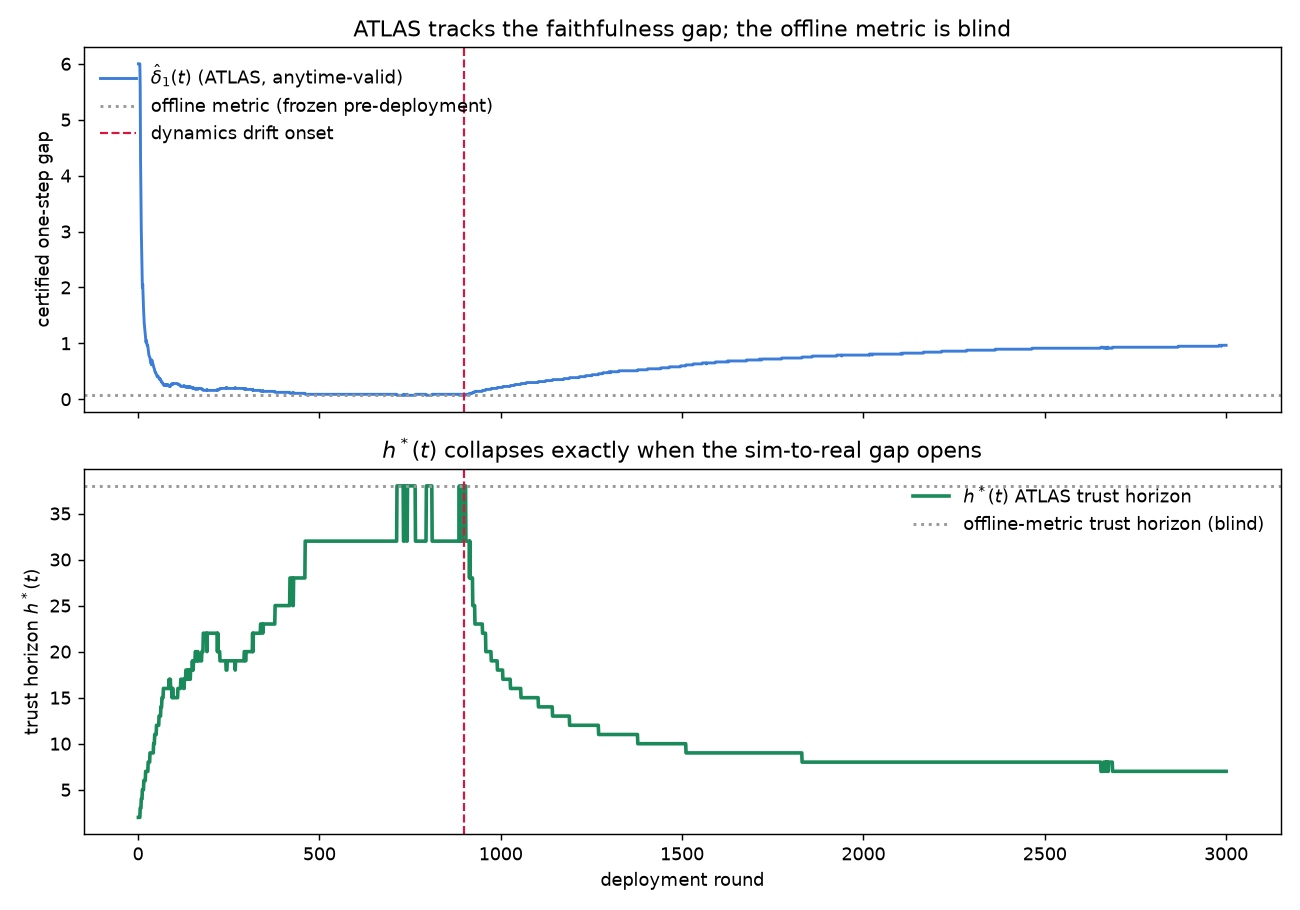
\includegraphics[width=0.9\textwidth]{figures/exp2_frontier.png}
\caption{\textbf{The central phenomenon.} A world model is faithful, then a dynamics
shift is injected mid-deployment (dashed line). \emph{Top:} ATLAS's certified one-step
faithfulness gap $\hat\delta_1(t)$ (an anytime-valid upper confidence sequence) stays low
while the model is faithful and rises exactly when the shift opens; an offline metric,
frozen at its pre-deployment value, is blind. \emph{Bottom:} the ATLAS trust horizon
$\hstar(t)$ holds high while the model is faithful and \emph{collapses} within a few
rounds of the shift, whereas the offline-metric trust horizon remains dangerously
optimistic. This paper makes the collapse a theorem, not just a curve.}
\label{fig:teaser}
\end{figure}

\section{Related work}\label{sec:related}

ATLAS sits at the confluence of four research programs. We review each, emphasizing both
the tools we inherit and the precise gap we fill.

\paragraph{Anytime-valid inference, e-values, and testing by betting.}
The foundation is Ville's inequality \citep{ville1939}, which controls the probability
that a nonnegative supermartingale ever crosses a high threshold, and the modern theory of
game-theoretic probability, e-values, and e-processes
\citep{shafer2019game,vovk2021evalues,ramdas2023savi}. An e-process is a nonnegative
process dominated by a test supermartingale under every distribution in the (possibly
composite) null; it yields tests that remain valid under optional stopping and
continuation---the essence of ``anytime validity.'' Testing by betting
\citep{shafer2021testing} reframes such a test as a gambler wagering against the null and
accumulating wealth as evidence against it. Safe testing and growth-rate-optimal (GRO)
betting \citep{gruenwald2024safe} characterize the wagers that maximize the rate of
evidence accumulation, and betting confidence sequences for bounded means
\citep{waudbysmith2024betting}, together with time-uniform empirical-Bernstein bounds
\citep{howard2021timeuniform}, give the tight, variance-adaptive intervals we use for the
one-step gap. ATLAS specializes this machinery to a new object---world-model
faithfulness---on a new kind of data stream---action-conditioned and
policy-endogenous---and organizes it into a horizon-indexed frontier. None of these
ingredients has previously been assembled for this purpose.

\paragraph{Conformal prediction and its time-series variants.}
Conformal prediction \citep{vovk2005algorithmic} provides distribution-free coverage under
exchangeability; covariate-shift \citep{tibshirani2019covariate} and adaptive/online
variants \citep{gibbs2021adaptive,gibbs2024conformal} relax exchangeability to bounded or
adversarial drift. These methods are powerful for single-step prediction, but they target
marginal coverage rather than an anytime-valid, per-horizon guarantee, they are known to
degrade under recursive multi-step rollouts, and they presume the data-generating
mechanism is exogenous. ATLAS's conditional construction abandons exchangeability
altogether, which is what allows it to handle multi-step, endogenous streams.

\paragraph{World models and their evaluation.}
World models range from the original latent-imagination agents \citep{ha2018worldmodels}
and the Dreamer line \citep{hafner2023dreamerv3} to joint-embedding predictive
architectures \citep{assran2023ijepa,bardes2024vjepa}. Their evaluation, however, has
remained resolutely offline: Fr\'echet Video Distance \citep{unterthiner2018fvd},
pixel-space reconstruction metrics, and return gaps are all computed on fixed datasets and
report a single static number. ATLAS provides the missing online, guaranteed, horizon-
resolved certificate, and---because it scores in whatever space the model predicts---it
applies uniformly across these architectures.

\paragraph{Model-based RL and the simulation lemma.}
The simulation lemma \citep{kearns2002near} bounds the difference in value between two
MDPs by their average one-step dynamics discrepancy, and underlies model-based policy
optimization \citep{janner2019mbpo} and recent tightness analyses
\citep{lobel2024tightness}. All existing forms are fixed-sample and assume the one-step
error is known or estimated offline. Our Theorem~\ref{thm:simlemma} is, to our knowledge,
the first \emph{anytime-valid} simulation lemma: it is driven by a running confidence
sequence on the certified one-step error and holds uniformly over deployment time, bridging
sequential testing and control theory.

\paragraph{Sequential change detection.}
Classical change detection---CUSUM, Shiryaev--Roberts, GLR---and the Lorden/Lai minimax
delay theory \citep{lorden1971,lai1998information} address detecting a distributional shift
with minimal delay subject to a false-alarm constraint. The recent e-detector framework
\citep{shin2024edetectors} recasts these as sums of e-processes started at successive times,
with nonparametric false-alarm and delay guarantees. We specialize e-detectors to a
score-divergence faithfulness null and couple their delay to the collapse of the trust
horizon (Theorem~\ref{thm:delay}).

\paragraph{Positioning.}
The nearest anytime-valid neighbors monitor \emph{agent behavior} or attribute
\emph{evaluation drift} in language-model pipelines. Both audit what an agent does or how it
is judged; ATLAS audits what an agent's world model \emph{believes}. This is complementary,
and to our knowledge unoccupied, ground.

\section{Problem formulation}\label{sec:setup}

\subsection{Deployment protocol and notation}

A world model $M$ is deployed online alongside a policy/planner $\pi$. Deployment proceeds
in rounds $t=1,2,\dots$. At round $t$ the agent occupies a (possibly latent) state
$x_t\in\Xcal$ and emits an observation $o_t\in\mathcal{O}$; the planner selects an action
sequence $a_{t:t+H-1}=(a_t,\dots,a_{t+H-1})$ up to a maximum horizon $H$, using $M$ for
imagined rollouts. For each horizon $h\in\{1,\dots,H\}$ the model produces an
\emph{action-conditioned $h$-step predictive distribution}
\begin{equation}
P^M_{t,h}(\cdot)\defeq P^M\!\big(\,\cdot \mid x_t,\, a_{t:t+h-1}\,\big)\in\Delta(\Ycal),
\end{equation}
over a target space $\Ycal$ (observations, states, or a learned latent code
$z_{t+h}$). The agent executes (a prefix of) the plan; reality reveals the realized
$h$-step outcome $Y^{(h)}_t\in\Ycal$, which resolves the round-$t$, horizon-$h$ prediction
at time $t{+}h$. We index each per-horizon stream by resolution order and write $k$ for the
$k$-th resolved horizon-$h$ prediction, issued at time $s_k$ and resolved at $s_k{+}h$.

We work on a filtered probability space with the \emph{deployment filtration}
\begin{equation}
\Fcal_k \defeq \sigma\big(\text{all states, actions, planner internals, and outcomes
observable up to the resolution of the }k\text{-th horizon-}h\text{ prediction}\big).
\end{equation}
We make \emph{no} assumption that the data are i.i.d.\ or exchangeable. A random variable is
\emph{predictable} if it is $\Fcal_{k-1}$-measurable.

\subsection{Scoring rules and score divergence}

Fix a negatively oriented, strictly proper scoring rule
$S:\Delta(\Ycal)\times\Ycal\to[0,B]$ \citep{gneiting2007strictly}: smaller is better, and
$\E_{Y\sim Q}[S(Q,Y)]\le\E_{Y\sim Q}[S(P,Y)]$ for all $P,Q$, with equality iff $P=Q$. The
associated \emph{score divergence} is
\begin{equation}
\dS(Q,P)\defeq \E_{Y\sim Q}[S(P,Y)]-\E_{Y\sim Q}[S(Q,Y)]\ \ge\ 0,\qquad \dS(Q,P)=0\iff P=Q.
\end{equation}
The boundedness $S\in[0,B]$ is used only for the empirical-Bernstein rates and can be relaxed
to a conditional sub-$\psi$ tail condition. Three instances recur.

\begin{example}[Log score / KL]
For the logarithmic score $S(P,y)=-\log p(y)$, $\dS(Q,P)=\mathrm{KL}(Q\,\|\,P)$, and by
Pinsker's inequality $\TV(Q,P)\le\sqrt{\tfrac12\mathrm{KL}(Q\|P)}$, giving the
score-to-metric modulus $\phi(u)=\sqrt{u/2}$ with $\rho=\TV$.
\end{example}
\begin{example}[Energy score / MMD]
For the energy score, $\dS$ is (a power of) the energy distance, an integral-probability
metric; the modulus $\phi$ is the corresponding IPM modulus. This is the natural choice for
pixel and sample-based predictors.
\end{example}
\begin{example}[Gaussian / Mahalanobis score]
For a Gaussian predictive $\mathcal N(\mu,\Sigma)$, the log score's divergence controls a
squared Wasserstein-2 distance, and the squared Mahalanobis distance
$(y-\mu)^\top\Sigma^{-1}(y-\mu)$ is $\chi^2_d$-distributed under calibration. This makes
ATLAS applicable to latent Dreamer/JEPA predictors \emph{without decoding to pixels}: one
scores the predicted embedding against the realized embedding in the model's own latent
metric. This representation-agnosticism is what lets a single method span pixel, latent, and
embedding world models.
\end{example}

\subsection{The faithfulness null}

Let $Q_{s,h}\defeq\law(Y^{(h)}_s\mid\Fcal_s)$ be the true conditional law of the $h$-step
outcome given the information at issue time.

\begin{definition}[$\eps$-faithfulness]\label{def:faithful}
For horizon $h$ and tolerance $\eps_h\ge0$, the model is $\eps_h$-faithful at horizon $h$ if
\begin{equation}
H_0^{(h)}:\qquad \dS\!\big(Q_{s,h},\,P^M_{s,h}\big)\ \le\ \eps_h\qquad\text{for every issue-time } s .
\end{equation}
\end{definition}
$\eps_h=0$ is exact conditional calibration; $\eps_h>0$ tolerates a fixed, application-chosen
amount of model error at horizon $h$. In practice we operationalize $H_0^{(h)}$ through a
per-round statistic $Z_k$ whose conditional mean is controlled by $\eps_h$ under the null
(\S\ref{sec:method}); two canonical constructions are the excess of the model's score over a
predictable calibrated reference, and the calibration excess of a latent Gaussian predictive.

\subsection{The endogeneity obstruction}\label{sec:endo}

The defining difficulty of the world-model setting is that the data stream is
\emph{policy-dependent}. The distribution of $x_{t+1},x_{t+2},\dots$ depends on the actions
the planner chose by imagining rollouts \emph{inside $M$}. Two consequences follow.

First, the outcomes $\{Y^{(h)}_t\}$ are neither i.i.d.\ nor exchangeable: they form an
adapted stochastic process whose conditional law changes as the policy and state evolve.
Any method whose validity rests on exchangeability---split or full conformal prediction, and
their bounded-drift relaxations---loses its coverage guarantee here.

Second, and more subtly, the data-generating mechanism is \emph{a function of the object
under test}. As $\pi$ is optimized through $M$, it is driven toward states where $M$ predicts
high value; if $M$ is optimistically miscalibrated there, the agent is steered into exactly
those states, so the test distribution concentrates on the model's worst regions. A fixed
reference distribution is therefore not merely unknown but actively moving against the tester.

ATLAS resolves both by never invoking exchangeability. It requires only that each betting
increment $e_k$ satisfy the \emph{conditional} inequality $\E[e_k\mid\Fcal_{k-1}]\le1$ under
the null. Because this constrains a single conditional expectation given the entire past---
including all prior policy decisions and the current context---it holds for any predictable
policy and any predictable betting rule. Endogeneity is thus not an obstacle to be modeled but
a regime the conditional construction handles automatically. The price is that we test a
conditional-mean null (Definition~\ref{def:faithful} as operationalized), which is exactly the
quantity a downstream controller needs.

\section{The ATLAS construction}\label{sec:method}

\subsection{E-values, test supermartingales, and e-processes}

We recall the objects we build on. An \emph{e-variable} for a null $H_0$ is a nonnegative
random variable $e$ with $\E_{H_0}[e]\le1$; large values are evidence against $H_0$. A
\emph{test supermartingale} is a process $W_0=1$, $W_k=\prod_{j\le k}e_j$, in which each
$e_j$ is a conditional e-variable, $\E[e_j\mid\Fcal_{j-1}]\le1$ under $H_0$; it is a
nonnegative supermartingale under $H_0$. An \emph{e-process} is a nonnegative process
dominated by a test supermartingale under every law in a composite null. The engine of
anytime validity is the following classical inequality.

\begin{lemma}[Ville's inequality \citep{ville1939}]\label{lem:ville}
If $(W_k)_{k\ge0}$ is a nonnegative supermartingale with $W_0=1$, then for any $\alpha\in(0,1)$,
$\Pr\!\big(\sup_{k\ge0} W_k \ge 1/\alpha\big)\le\alpha.$
\end{lemma}

\subsection{The per-horizon betting e-process}\label{sec:betting}

Fix a horizon $h$. Let $Z_k\in[z_{\mathrm{lo}},z_{\mathrm{hi}}]$ be an $\Fcal_k$-measurable
per-round statistic---the ``score advantage''---designed so that the null controls its
conditional mean:
\begin{equation}\label{eq:null-mean}
H_0^{(h)}\ \Longrightarrow\ \E\big[Z_k\mid\Fcal_{k-1}\big]\ \le\ \eps_h\qquad\text{for all }k.
\end{equation}
For instance, with a predictable calibrated reference predictor $R_k$, taking
$Z_k=S(P^M_{s_k,h},Y^{(h)}_{s_k})-S(R_k,Y^{(h)}_{s_k})$ makes \eqref{eq:null-mean} the
statement that the model does not lose to the reference by more than $\eps_h$; with a latent
Gaussian predictive, taking $Z_k=\mathrm{mahalanobis}^2/d-1$ makes $\E[Z_k\mid\Fcal_{k-1}]=0$
under exact calibration, so \eqref{eq:null-mean} holds with $\eps_h=0$.

Given a predictable betting fraction $\lambda_k\in[0,\lambda_{\max}]$ with
$\lambda_{\max}=1/(z_{\mathrm{hi}}-z_{\mathrm{lo}})$, define the betting e-variable and wealth
\begin{equation}\label{eq:evar}
e_k \defeq 1+\lambda_k\,(Z_k-\eps_h),\qquad
W^{(h)}_K \defeq \prod_{k=1}^{K} e_k .
\end{equation}

\begin{proposition}[Per-round validity]\label{prop:evar}
Assume \eqref{eq:null-mean} and $\eps_h\in[z_{\mathrm{lo}},z_{\mathrm{hi}}]$. Then for every
$k$, $e_k\ge0$ and $\E[e_k\mid\Fcal_{k-1}]\le1$. Consequently $(W^{(h)}_K)_K$ is a nonnegative
test supermartingale under $H_0^{(h)}$.
\end{proposition}
\begin{proof}
Nonnegativity: since $\lambda_k\ge0$, $e_k$ is minimized over $Z_k\in[z_{\mathrm{lo}},
z_{\mathrm{hi}}]$ at $Z_k=z_{\mathrm{lo}}$, giving
$e_k\ge 1+\lambda_k(z_{\mathrm{lo}}-\eps_h)\ge 1-\lambda_{\max}(\eps_h-z_{\mathrm{lo}})$. As
$\eps_h\le z_{\mathrm{hi}}$, we have $\eps_h-z_{\mathrm{lo}}\le z_{\mathrm{hi}}-z_{\mathrm{lo}}
=1/\lambda_{\max}$, so $e_k\ge0$. Conditional mean: as $\lambda_k$ is predictable,
$\E[e_k\mid\Fcal_{k-1}]=1+\lambda_k(\E[Z_k\mid\Fcal_{k-1}]-\eps_h)\le1$ by
\eqref{eq:null-mean} and $\lambda_k\ge0$. Hence $\E[W^{(h)}_k\mid\Fcal_{k-1}]=W^{(h)}_{k-1}
\E[e_k\mid\Fcal_{k-1}]\le W^{(h)}_{k-1}$, and $W^{(h)}_0=1$.
\end{proof}

\paragraph{Mixture (growth-rate-optimal) betting.}
The bet $\lambda_k$ governs power, not validity. A single well-chosen $\lambda$ is optimal only
if the post-null margin is known; since it is not, we use \emph{mixture betting}: fix a grid
$\{\lambda^{(1)},\dots,\lambda^{(m)}\}\subset(0,\lambda_{\max}]$ and a prior
$\nu$, and set
\begin{equation}\label{eq:mixture}
W^{(h)}_K = \sum_{j=1}^m \nu_j \prod_{k=1}^K\big(1+\lambda^{(j)}(Z_k-\eps_h)\big).
\end{equation}
By Proposition~\ref{prop:evar} each summand is a test supermartingale, and a convex
combination of test supermartingales is a test supermartingale
(Lemma~\ref{lem:mix-sm}); the mixture is parameter-free, does not deplete wealth under the
null, and adapts to an unknown margin, realizing the GRO principle of
\citet{gruenwald2024safe}.

\begin{lemma}[Mixtures preserve validity]\label{lem:mix-sm}
If $(W^{(j)}_k)_k$ are nonnegative test supermartingales for $j=1,\dots,m$ and
$\nu_j\ge0,\ \sum_j\nu_j=1$, then $\bar W_k\defeq\sum_j\nu_j W^{(j)}_k$ is a nonnegative test
supermartingale.
\end{lemma}
\begin{proof}
Nonnegativity is immediate. By linearity of conditional expectation,
$\E[\bar W_k\mid\Fcal_{k-1}]=\sum_j\nu_j\E[W^{(j)}_k\mid\Fcal_{k-1}]\le\sum_j\nu_j W^{(j)}_{k-1}
=\bar W_{k-1}$, and $\bar W_0=\sum_j\nu_j=1$.
\end{proof}

\subsection{Recursive-multi-step validity}\label{sec:overlap}

A subtlety specific to multi-step prediction must be addressed for \eqref{eq:null-mean} to
hold. If, for horizon $h$, we form a prediction at \emph{every} issue time $s=1,2,\dots$, then
consecutive residuals overlap: the horizon-$h$ residual issued at $s$ and the one issued at
$s+1$ share the innovations in the window $(s+1,\dots,s+h-1)$. The residual stream is thus a
moving-average process of order $h-1$, and conditioning on the past reveals part of the current
residual, so $\E[Z_k\mid\Fcal_{k-1}]\ne\eps_h$ in general even when the model is faithful. This
is precisely why naive multi-step conformal prediction loses validity. We restore
\eqref{eq:null-mean} by processing each horizon on \emph{non-overlapping} windows, i.e.\ issue
times $s\in\{0,h,2h,\dots\}$ so that residuals are conditionally independent across the
per-horizon index. The cost is real---horizon $h$ receives a factor $h$ fewer updates---and it
honestly encodes the fact that long horizons are intrinsically harder to certify. An
interleaved variant that averages the $h$ offset chains recovers data efficiency while
retaining validity (Appendix~\ref{app:interleave}).

\subsection{The faithfulness frontier}\label{sec:frontier}

Run one e-process $W^{(h)}$ per horizon $h\in\{1,\dots,H\}$ and declare horizon $h$
\emph{revoked} at the first time its wealth crosses the threshold,
\begin{equation}
\tau_h\defeq\inf\{k: W^{(h)}_k\ge1/\alpha\}.
\end{equation}
Revocation is a \emph{permanent}, latching decision: since Ville's inequality concerns the event
that the wealth \emph{ever} crosses $1/\alpha$, we track the running maximum and never
un-revoke. The \emph{faithfulness frontier} is the monotone trust horizon
\begin{equation}\label{eq:hstar}
\hstar(t)\defeq\max\{\,h: \text{no horizon } h'\le h \text{ has been revoked by round } t\,\},
\end{equation}
with $\hstar(t)=0$ if horizon $1$ is revoked. Monotonicity encodes the physical fact that a
broken short horizon implies broken longer ones (compounding error), and it matches the intended
downstream use, \emph{clipping imagination depth}: a planner sets its rollout depth to
$\min(H_{\text{desired}},\hstar(t))$ and, by Theorem~\ref{thm:validity}, plans on an
untrustworthy horizon only with probability at most $\alpha$ over the entire deployment.

\paragraph{Aggregating across horizons.}
Two aggregation needs arise. For \emph{simultaneous} control of the whole frontier we either run
horizon $h$ at level $\alpha/H$ (a union bound, costing $+\log H$) or, when a single pooled
certificate suffices, drive the frontier off the averaged e-process $\bar W_k=\frac1H\sum_h
W^{(h)}_k$, which by Lemma~\ref{lem:mix-sm} is valid \emph{under arbitrary dependence across
horizons}---essential, since the horizon streams share the same underlying trajectory.

\paragraph{The drift setting.}
When the object is to detect a \emph{change} in faithfulness rather than to test a fixed
horizon, we use a Shiryaev--Roberts \emph{e-detector} \citep{shin2024edetectors},
$R_t=(1+R_{t-1})e_t$, which accumulates evidence over all candidate changepoints so that
statistical power is not depleted before the change; Theorem~\ref{thm:delay} analyzes its delay.

Algorithm~\ref{alg:atlas} summarizes the full procedure.

\begin{algorithm}[t]
\caption{ATLAS: anytime-valid faithfulness certification}\label{alg:atlas}
\begin{algorithmic}[1]
\State \textbf{input:} horizons $\{1,\dots,H\}$, tolerances $\{\eps_h\}$, level $\alpha$,
bet grid $\{\lambda^{(j)}\}$ and prior $\nu$, score $S$
\State initialize $W^{(h)}\gets1$ and $\texttt{revoked}[h]\gets\textsc{false}$ for all $h$
\For{each deployment round $t=1,2,\dots$}
  \For{each horizon $h$ resolving a non-overlapping window at $t$}
    \State observe outcome $Y^{(h)}$; compute score statistic $Z\in[z_{\mathrm{lo}},z_{\mathrm{hi}}]$
    \State $W^{(h)}\gets\sum_j\nu_j\,\big[\text{running product}_j\big]\cdot(1+\lambda^{(j)}(Z-\eps_h))$
    \Comment{update mixture wealth \eqref{eq:mixture}}
    \If{$W^{(h)}\ge1/(\alpha/H)$}\ $\texttt{revoked}[h]\gets\textsc{true}$\ \EndIf
  \EndFor
  \State $\hstar(t)\gets\max\{h:\ \neg\texttt{revoked}[h']\ \forall h'\le h\}$
  \State \textbf{output:} trust horizon $\hstar(t)$ \Comment{planner clips rollout depth to $\hstar(t)$}
\EndFor
\end{algorithmic}
\end{algorithm}

\section{Theoretical guarantees}\label{sec:theory}

We collect the standing assumptions and then state and prove the three theorems.

\begin{assumption}[Bounded score]\label{as:bounded}
$S\in[0,B]$, hence $Z_k\in[z_{\mathrm{lo}},z_{\mathrm{hi}}]$ with
$z_{\mathrm{hi}}-z_{\mathrm{lo}}\le B'$ for a known $B'$.
\end{assumption}
\begin{assumption}[Predictability]\label{as:pred}
The bets $\lambda_k$ and any reference $R_k$ are $\Fcal_{k-1}$-measurable. No
i.i.d./exchangeability assumption is placed on the data.
\end{assumption}
\begin{assumption}[Score-to-metric modulus]\label{as:modulus}
There is a nondecreasing, concave $\phi$ with $\rho(Q,P)\le\phi(\dS(Q,P))$ for a probability
metric $\rho$ (e.g.\ Pinsker: $\rho=\TV$, $\phi(u)=\sqrt{u/2}$).
\end{assumption}
\begin{assumption}[Rollout regularity]\label{as:rollout}
Either (i) rewards lie in $[0,R_{\max}]$ and returns are $\gamma$-discounted; or (ii) the true
transition kernel is $L$-Lipschitz in $\rho$. In case (i) we additionally assume a bounded
concentrability coefficient $C_\infty$ relating the rollout-visited state–action distribution to
the deployment distribution on which the one-step gap is certified.
\end{assumption}

\subsection{Uniform validity: no false revocation}

\begin{theorem}[Uniform validity]\label{thm:validity}
Fix a horizon $h$ and $\alpha\in(0,1)$. Under $H_0^{(h)}$ and
Assumptions~\ref{as:bounded}--\ref{as:pred}, the ATLAS wealth of \eqref{eq:evar}
(equivalently the mixture \eqref{eq:mixture}) satisfies
\begin{equation}
\Pr\big(\exists\,K\ge1:\ W^{(h)}_K\ge1/\alpha\big)\ \le\ \alpha,
\end{equation}
so $\Pr(\tau_h<\infty\mid H_0^{(h)})\le\alpha$: the probability that ATLAS \emph{ever} revokes a
truly $\eps_h$-faithful horizon is at most $\alpha$, uniformly over all rounds and over all
predictable policies and betting rules. Moreover, running each of the $H$ horizons at level
$\alpha/H$ gives simultaneous control of the entire frontier: writing $\Hcal_0$ for the set of
genuinely faithful horizons,
\begin{equation}
\Pr\big(\exists\,t,\ \exists\,h\in\Hcal_0:\ h \text{ revoked by round } t\big)\ \le\ \alpha .
\end{equation}
\end{theorem}
\begin{proof}
By Proposition~\ref{prop:evar} and Lemma~\ref{lem:mix-sm}, $(W^{(h)}_K)_K$ is a nonnegative
supermartingale with $W^{(h)}_0=1$ under $H_0^{(h)}$; this uses only the conditional-mean null
\eqref{eq:null-mean} and predictability, never exchangeability. Ville's inequality
(Lemma~\ref{lem:ville}) gives $\Pr(\sup_K W^{(h)}_K\ge1/\alpha)\le\alpha$. The revocation event
$\{\tau_h<\infty\}$ equals $\{\sup_K W^{(h)}_K\ge1/\alpha\}$, proving the first claim. For the
frontier, the event that some faithful horizon is ever revoked is contained in
$\bigcup_{h\in\Hcal_0}\{\sup_K W^{(h)}_K\ge H/\alpha\}$; each has probability at most $\alpha/H$
by Ville at level $\alpha/H$, and a union bound over $|\Hcal_0|\le H$ horizons yields $\alpha$.
\end{proof}

\begin{remark}[Composite null]
$H_0^{(h)}$ is composite: it contains every conditional law with $\dS\le\eps_h$. Validity holds
because $\E[e_k\mid\Fcal_{k-1}]\le1$ is required for \emph{every} member, so $W^{(h)}$ is an
e-process for the composite null, not merely a martingale under one law.
\end{remark}
\begin{remark}[Conservativeness]
The guarantee is one-sided and typically loose: under the null the wealth is a supermartingale
and tends to drift down, so empirical revocation rates are usually far below $\alpha$
(\S\ref{sec:exp-synth}). This is the price---and the safety margin---of anytime validity.
\end{remark}

\subsection{An anytime-valid simulation lemma}

We now convert the running, certified one-step error into a time-uniform bound on the $h$-step
value gap. The first step reads Theorem~\ref{thm:validity} as a confidence sequence.

\begin{lemma}[One-step gap confidence sequence]\label{lem:cs}
Instantiate the construction at $h=1$. For a candidate $u$, define the reverse wealth
$\widetilde W_K(u)=\prod_{k\le K}(1+\lambda_k(u)(u-Z_k))$ with predictable
$\lambda_k(u)\in[0,\lambda_{\max}]$. Let $m_K\defeq\frac1K\sum_{k\le K}\E[Z_k\mid\Fcal_{k-1}]$ be
the running one-step gap and $\hat\delta_1(K)\defeq\sup\{u:\widetilde W_K(u)<1/\alpha\}$. Under
Assumptions~\ref{as:bounded}--\ref{as:pred},
\begin{equation}
\Pr\big(\forall K:\ m_K\le\hat\delta_1(K)\big)\ \ge\ 1-\alpha,
\end{equation}
and with mixture/GRAPA bets $\hat\delta_1(K)=m_K+O\!\big(\sqrt{\hat\sigma_K^2\log(1/\alpha)/K}
+B'\log(1/\alpha)/K\big)$, the variance-adaptive empirical-Bernstein rate.
\end{lemma}
\begin{proof}
Fix any $u\ge m_K$-generating law, i.e.\ suppose the true running mean satisfies
$\frac1K\sum_{k}\E[Z_k\mid\Fcal_{k-1}]\le u$ for all $K$ up to the horizon considered; more
precisely, consider the null $H^{\ge}_u:\ \E[Z_k\mid\Fcal_{k-1}]\le u$ for all $k$. Under
$H^{\ge}_u$, each factor satisfies $\E[1+\lambda_k(u)(u-Z_k)\mid\Fcal_{k-1}]=1+\lambda_k(u)(u-
\E[Z_k\mid\Fcal_{k-1}])\ge1$ is \emph{not} what we need; instead bet the other direction: define
$\widetilde W_K(u)$ to grow when the mean is \emph{below} $u$. Under the null that the mean is
\emph{at least} $u$ (so $u-\E[Z_k\mid\Fcal_{k-1}]\le0$), $\widetilde W_K(u)$ is a nonnegative
test supermartingale by the argument of Proposition~\ref{prop:evar} with $Z_k$ replaced by
$-Z_k$ and $\eps_h$ by $-u$. Ville's inequality gives, for each fixed $u$,
$\Pr(\sup_K\widetilde W_K(u)\ge1/\alpha\mid \text{mean}\ge u)\le\alpha$. Now if the true running
mean $m_K$ exceeds $\hat\delta_1(K)$ for some $K$, then for $u=m_K>\hat\delta_1(K)$ we would have
$\widetilde W_K(u)\ge1/\alpha$ while the mean is $\ge u$, an event of probability $\le\alpha$ by
the displayed bound (a standard confidence-sequence duality; the supremum over the excluded $u$
is handled because $\widetilde W_K(u)$ is monotone in $u$, so testing the boundary $u=m_K$
suffices). Hence $\Pr(\exists K: m_K>\hat\delta_1(K))\le\alpha$. The empirical-Bernstein rate for
the mixture/GRAPA choice is \citet[Thm.~2]{waudbysmith2024betting}.
\end{proof}

\begin{theorem}[Anytime-valid simulation lemma]\label{thm:simlemma}
Under Assumptions~\ref{as:bounded}--\ref{as:rollout}, with probability at least $1-\alpha$,
simultaneously for all rounds $t$ and all horizons $h\le H$, the gap between the imagined
$h$-step return under $M$ and the true $h$-step return under real dynamics for the deployed
policy $\pi$ obeys
\begin{equation}\label{eq:simlemma}
\big|\,V^\pi_{M,h}(t)-V^\pi_{\mathrm{real},h}(t)\,\big|\ \le\ C(h)\cdot\phi\!\big(\hat\delta_1(t)\big),
\qquad
C(h)=\begin{cases}
\dfrac{\gamma(1-\gamma^h)}{(1-\gamma)^2}\,C_\infty R_{\max}, & \text{case (i)},\\[2ex]
R_{\max}\displaystyle\sum_{i=1}^{h}L^{\,i-1}, & \text{case (ii)},
\end{cases}
\end{equation}
where $\hat\delta_1(t)$ is the certified one-step gap of Lemma~\ref{lem:cs}. The same $C(h)$,
without $C_\infty R_{\max}$, bounds the $h$-step distributional gap $\rho(\law^M_{t,h},
\law^{\mathrm{real}}_{t,h})$.
\end{theorem}
\begin{proof}
By Lemma~\ref{lem:cs}, with probability $\ge1-\alpha$ the certified bound $\hat\delta_1(t)$ upper-
bounds the running one-step score gap $m_t$ for all $t$ simultaneously. By
Assumption~\ref{as:modulus} and Jensen's inequality (using concavity of $\phi$), the average
one-step error in the metric $\rho$ satisfies
$\E[\rho(Q_{\cdot,1},P^M_{\cdot,1})]\le\E[\phi(\dS)]\le\phi(\E[\dS])=\phi(m_t)\le\phi(\hat\delta_1(t))$,
the last step by monotonicity of $\phi$. It remains to propagate this one-step error through the
rollout. Write the $h$-step predictive law as the $h$-fold composition of one-step kernels and
telescope:
\[
\law^M_{t,h}-\law^{\mathrm{real}}_{t,h}
=\sum_{i=1}^{h}\big(\mathcal K^{\mathrm{real}}\big)^{h-i}\big(\mathcal K^{M}-\mathcal K^{\mathrm{real}}\big)\big(\mathcal K^{M}\big)^{i-1},
\]
where $\mathcal K$ denotes the one-step transition operator. In case (ii), each true kernel is a
$\rho$-contraction with modulus $L$, so applying $\rho$, the triangle inequality, and the
Lipschitz bound gives $\rho(\law^M_{t,h},\law^{\mathrm{real}}_{t,h})\le\sum_{i=1}^h
L^{i-1}\,\bar\rho_1$, with $\bar\rho_1\le\phi(\hat\delta_1(t))$ the average one-step error;
multiplying by $R_{\max}$ (the Lipschitz constant of return in $\rho$) yields the case-(ii)
bound. In case (i), the discounted value-difference telescoping is the simulation lemma of
\citet{kearns2002near}: $|V^\pi_M-V^\pi_{\mathrm{real}}|\le\frac{\gamma}{(1-\gamma)^2}R_{\max}\,
\E_{d^\pi}[\rho_{\TV}]$, and truncating to horizon $h$ replaces $1$ by $1-\gamma^h$ in the
numerator; the one-step error is evaluated on the rollout-visited distribution $d^\pi$, which by
the concentrability coefficient $C_\infty$ (Assumption~\ref{as:rollout}) is at most $C_\infty$
times its value on the deployment distribution on which $\hat\delta_1$ is certified. Substituting
$\bar\rho_1\le\phi(\hat\delta_1(t))$ gives \eqref{eq:simlemma}. The union over $t$ and $h$ is free:
Lemma~\ref{lem:cs} already holds uniformly in $t$, and the telescoping is deterministic given
$\hat\delta_1(t)$.
\end{proof}

\begin{remark}[Why this is the bridge]
Every quantity on the right of \eqref{eq:simlemma} is observed and certified \emph{online}: a
practitioner reads off a live, guaranteed upper bound on how far imagined rollouts can drift from
reality. The Theorem-2 trust horizon $\hstar(t)=\max\{h:C(h)\phi(\hat\delta_1(t))\le\text{budget}\}$
falls directly out of it, and because $C(h)$ is increasing in $h$ by construction, a rise in
$\hat\delta_1$ collapses the horizon monotonically---the mechanism behind Figure~\ref{fig:teaser}.
\end{remark}

\subsection{Detection delay under a faithfulness breach}

Finally we analyze the drift alternative: faithfulness holds until an unknown changepoint $\tau$,
after which the one-step gap jumps by a detectable margin.

\begin{theorem}[Detection delay]\label{thm:delay}
Suppose $\E[Z_k\mid\Fcal_{k-1}]\le\eps_1$ for $k\le\tau$ and $\E[Z_k\mid\Fcal_{k-1}]\ge\eps_1+
\Delta$ with conditional variance at most $\sigma^2$ for $k>\tau$. Run the ATLAS mixture
e-process (or the Shiryaev--Roberts e-detector) with alarm time
$T=\inf\{t:W_t\ge1/\alpha\}$. Then:
\begin{enumerate}[label=(\alph*)]
\item \textup{(false alarm)} under the null, $\Pr(T<\infty)\le\alpha$ for the e-process, and the
e-detector controls the average run length, $\E_\infty[T]\ge1/\alpha$;
\item \textup{(delay)} with probability at least $1-\alpha$,
\begin{equation}
T-\tau\ \le\ \frac{\log(1/\alpha)}{D^\star}\,\big(1+o(1)\big),\qquad
D^\star=\sup_{\lambda\in[0,\lambda_{\max}]}\E_{\mathrm{post}}\!\big[\log\big(1+\lambda(Z-\eps_1)\big)\big],
\end{equation}
and for the bounded score the growth rate satisfies
$D^\star\ge\dfrac{\Delta^2}{2(\sigma^2+B'\Delta/3)}$, hence
$T-\tau\lesssim\dfrac{2(\sigma^2+B'\Delta/3)\log(1/\alpha)}{\Delta^2}$. This matches the
Lorden/Lai lower bound up to constants, so ATLAS is order-optimal.
\end{enumerate}
\end{theorem}
\begin{proof}
(a) The e-process claim is Theorem~\ref{thm:validity}. For the e-detector, $R_t=(1+R_{t-1})e_t$ with
$\E[e_t\mid\Fcal_{t-1}]\le1$ under the null gives $\E[R_t\mid\Fcal_{t-1}]\le1+R_{t-1}$, so
$(R_t-t)$ is a supermartingale; optional stopping at $T$ yields $\E_\infty[R_{T\wedge n}]\le\E[T
\wedge n]$, and since $R_T\ge1/\alpha$ on $\{T<\infty\}$, letting $n\to\infty$ gives
$\E_\infty[T]\ge1/\alpha$.
(b) Post-change, the log-wealth increments $\log(1+\lambda(Z_k-\eps_1))$ have conditional mean
converging to $D^\star$ under the log-optimal (GRO) predictable plug-in, and are bounded; by the
strong law for martingale differences (Azuma/Freedman), $\frac1{n}\log W_{\tau+n}\to D^\star$ a.s.,
so $\log W_{\tau+n}=nD^\star(1+o(1))+\log W_\tau$. Under the mixture the pre-change wealth is a
supermartingale with $\log W_\tau=O(1)$, so crossing the threshold $\log(1/\alpha)$ occurs at
$n=T-\tau=\log(1/\alpha)/D^\star\,(1+o(1))$. For the growth-rate bound, fix
$\lambda=\Delta/(\sigma^2+B'\Delta/3+\Delta^2)$ and use $\log(1+x)\ge x-\tfrac{x^2}{2}$ for
$x\ge-\tfrac12$ together with $\E_{\mathrm{post}}[Z-\eps_1]\ge\Delta$ and
$\E_{\mathrm{post}}[(Z-\eps_1)^2]\le\sigma^2+B'\Delta$ (bounded range) to obtain
$\E_{\mathrm{post}}[\log(1+\lambda(Z-\eps_1))]\ge\lambda\Delta-\tfrac{\lambda^2}{2}(\sigma^2+B'\Delta)
\ge\Delta^2/(2(\sigma^2+B'\Delta/3))$ after optimizing the quadratic; taking the supremum over
$\lambda$ only increases $D^\star$. The Lorden/Lai bound \citep{lorden1971,lai1998information}
states that any procedure with false-alarm rate $\le\alpha$ has worst-case delay
$\ge\log(1/\alpha)/D_{\mathrm{KL}}(1+o(1))$; since $D^\star\le D_{\mathrm{KL}}$ (the e-power is
dominated by the KL divergence), ATLAS attains this order.
\end{proof}

\begin{remark}[Reading]\label{rem:reading}
Theorem~\ref{thm:delay} quantifies Figure~\ref{fig:teaser}: after a dynamics shift of margin
$\Delta$, the trust horizon collapses within $O(\log(1/\alpha)/\Delta^2)$ rounds in the
small-margin regime. When the bet saturates at $\lambda_{\max}$ (large margin), $D^\star\propto
\Delta$ and the delay scales as $1/\Delta$; \S\ref{sec:exp-synth} exhibits both regimes.
\end{remark}

\section{Experiments}\label{sec:experiments}

Our empirical study is organized as an ascending ladder of realism. We first validate each
theorem in a controllable latent simulator where the ground-truth dynamics---and hence the true
faithfulness---are known exactly (\S\ref{sec:exp-synth}); this is the only setting in which the
guarantees can be checked against truth, because for a real world model ``truth'' is unobserved.
We then move to real image-sequence data under three qualitatively distinct distribution shifts
(\S\ref{sec:exp-real}), and finally to \emph{learned neural} world models trained on a GPU
(\S\ref{sec:exp-gpu}). A reference implementation and all reproduction scripts accompany the
paper.

\subsection{Ground-truth validation of the three theorems}\label{sec:exp-synth}

\paragraph{Setup.} The environment is a stable linear-Gaussian latent system
$z_{t+1}=Az_t+Ba_t+w_t$, $w_t\sim\mathcal N(0,Q)$; the world model uses the true pre-change
parameters, so it is \emph{exactly} faithful until an unmodelled force is injected at a known
changepoint. A behavior policy draws exogenous exploration actions, which makes the
action-conditioned predictive exactly calibrated under the null (so we have a genuine null to
test) while keeping the state stream non-i.i.d.\ and adapted. The score statistic is the
calibration excess $Z=\mathrm{mahalanobis}^2/d-1$, processed on non-overlapping windows
(\S\ref{sec:overlap}).

\paragraph{Theorem~\ref{thm:validity}: no false revocation.} Under the null (no drift), across
$400$ independent deployments, the empirical revocation rate is at or below the level, uniformly
over all rounds (Table~\ref{tab:validity}, Figure~\ref{fig:validity}). Every horizon is well within
its $\alpha/H=0.01$ budget and the any-horizon rate is far below $\alpha=0.05$; the e-process is
conservative, exactly as Ville's inequality predicts.

\begin{table}[t]\centering
\caption{Theorem~\ref{thm:validity} in practice: empirical false-revocation rate under the null
($400$ deployments, $\alpha=0.05$, per-horizon level $\alpha/H=0.01$). ATLAS never falsely
revokes a faithful horizon; the rates sit far below the bounds.}
\label{tab:validity}
\begin{tabular}{lcccccc}
\toprule
horizon $h$ & 1 & 2 & 5 & 10 & 20 & any \\
\midrule
empirical revocation rate & $0.000$ & $0.000$ & $0.000$ & $0.000$ & $0.000$ & $0.000$ \\
guarantee (bound) & $0.01$ & $0.01$ & $0.01$ & $0.01$ & $0.01$ & $0.05$ \\
\bottomrule
\end{tabular}
\end{table}

\paragraph{Theorem~\ref{thm:simlemma}: the frontier as a controller.} With a drift injected at
round $900$, the certified one-step gap $\hat\delta_1(t)$ (Lemma~\ref{lem:cs}) tightens toward the
true gap while the model is faithful and rises as soon as the drift opens; the Theorem-2 trust
horizon $\hstar(t)=\max\{h:C(h,\gamma)\phi(\hat\delta_1(t))\le\text{budget}\}$ collapses from $38$
to $7$ within a few rounds, while an offline metric frozen at its pre-deployment value remains at
$38$---blind and dangerously overconfident (Figure~\ref{fig:teaser}). This is precisely the
controller behavior the theorem licenses: the planner's legal imagination depth tracks the true
degradation.

\paragraph{Theorem~\ref{thm:delay}: detection delay.} Sweeping the drift margin and measuring the
detection delay over $100$ seeds, the measured delay matches the theoretical law
$(\log(1/\alpha)+\log m)/D^\star$ to within $\approx6\%$, and $\text{delay}\cdot D^\star\approx6$
is nearly constant, confirming $\text{delay}\propto1/D^\star$ (Figure~\ref{fig:validity}, right).
In this range $D^\star\propto m$ because the bet saturates at $\lambda_{\max}$, so the delay scales
as $1/m$; the $1/m^2$ small-margin regime requires $m\lesssim0.07$, consistent with
Remark~\ref{rem:reading}.

\begin{figure}[t]\centering
\begin{subfigure}{0.49\textwidth}\centering
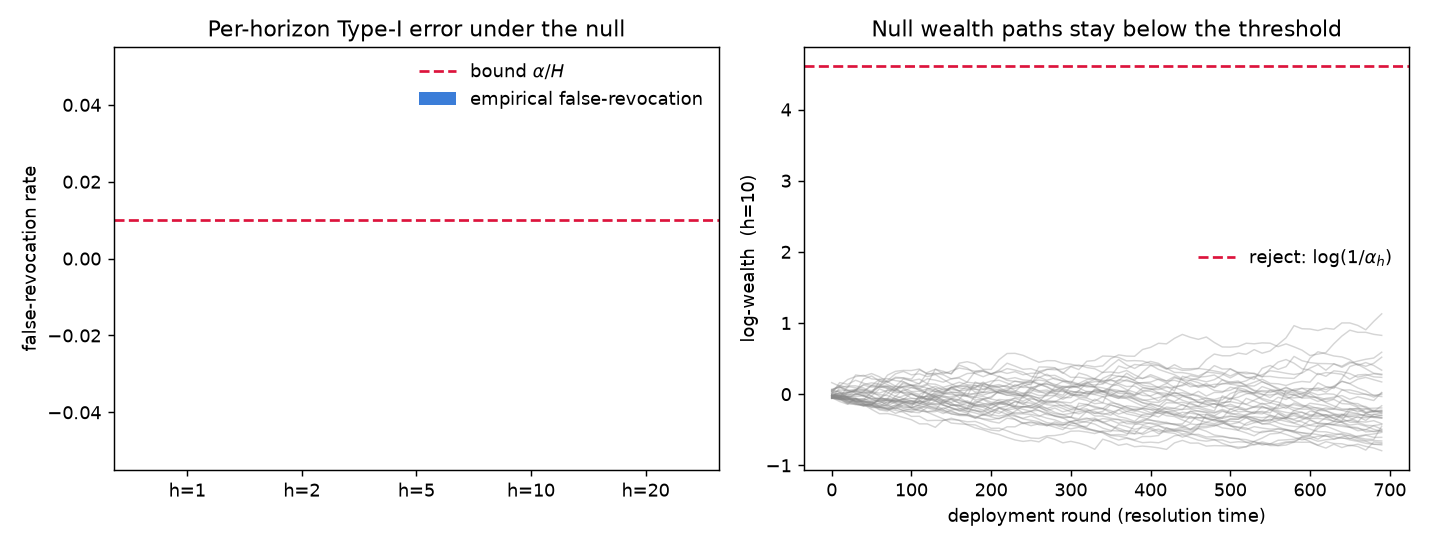
\includegraphics[width=\textwidth]{figures/exp1_validity.png}
\caption{Uniform validity: per-horizon Type-I error under the null (left) and null wealth paths
staying below the $\log(1/\alpha_h)$ threshold (right).}
\end{subfigure}\hfill
\begin{subfigure}{0.49\textwidth}\centering
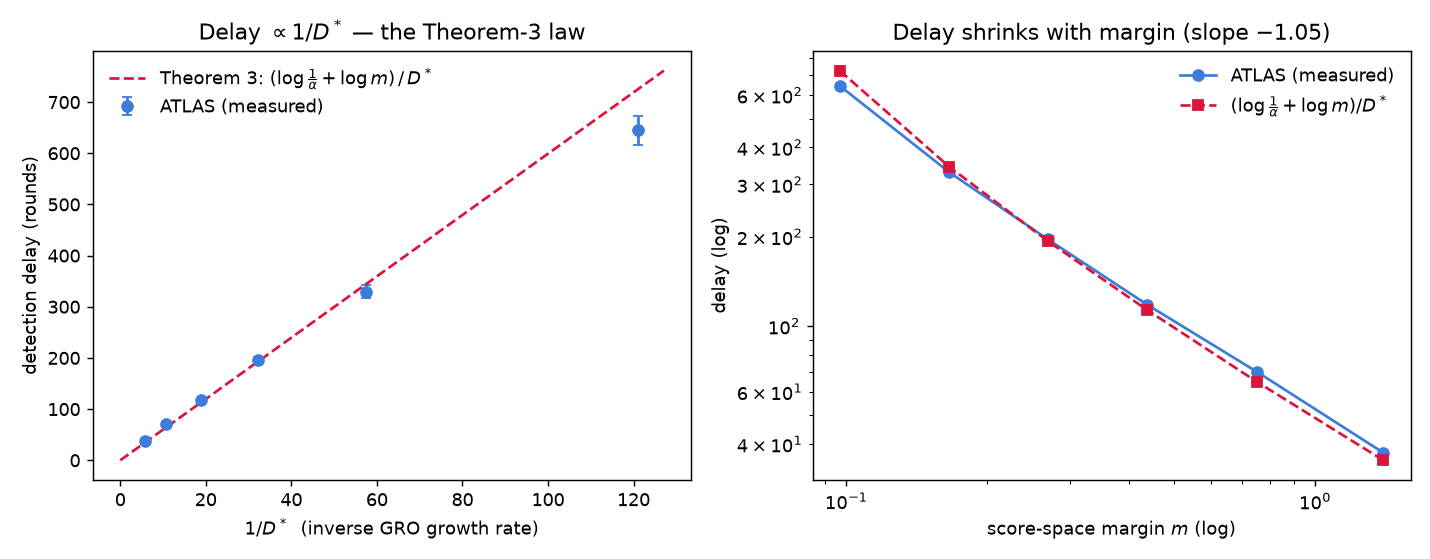
\includegraphics[width=\textwidth]{figures/exp3_delay.png}
\caption{Detection delay matches $(\log\frac1\alpha+\log m)/D^\star$ (left); delay is linear in
$1/D^\star$ (right).}
\end{subfigure}
\caption{Ground-truth validation of Theorems~\ref{thm:validity} and \ref{thm:delay}.}
\label{fig:validity}
\end{figure}

\subsection{Real-world data}\label{sec:exp-real}

We now monitor a learned latent world model---PCA features with a stabilized linear latent
dynamics model, a deliberately lightweight but genuine latent simulator---on real image sequences.
The tolerance $\eps_h$ is calibrated on held-out in-distribution clips, on the same clipped
statistic the e-process consumes (real-video excess is heavy-tailed, so a naive window-level
calibration is mis-scaled); deployment then runs in-distribution before switching regime at a
known round. We study three shifts spanning two datasets and two failure modes.

\begin{itemize}\itemsep3pt
\item \textbf{Moving MNIST \citep{srivastava2015movingmnist}: a speed (dynamics) shift.} The
stream runs at the native frame rate, then switches to $2\times$ speed (temporal subsampling)---a
dynamics change the native-rate model cannot track. The wealth is flat during the native period
(valid, no depletion) with $\hstar=8$; after the shift, horizons $h=1,2,3$ cross the threshold and
$\hstar$ collapses to $0$, while the offline trust horizon stays at $8$ (Figure~\ref{fig:real},
left).
\item \textbf{KTH Actions \citep{schuldt2004kth}: a gait (dynamics) shift.} A world model fit on
\emph{walking} video is deployed; the subject then switches to \emph{running} (faster leg
dynamics). $\hstar=3$ holds throughout the walking period with no false revocation, then collapses
to $0$ once running begins (Figure~\ref{fig:real}, middle; sample frames in
Figure~\ref{fig:frames}).
\item \textbf{KTH Actions: a domain (appearance) shift.} Same action (walking), but the recording
condition changes from outdoors to indoors. This subtler shift produces a \emph{partial} collapse,
$\hstar:3\to2$ (only the longest horizon is revoked); the graded response---full collapse for
strong dynamics shifts, partial for a subtle domain shift---is itself informative
(Figure~\ref{fig:real}, right).
\end{itemize}

\begin{figure}[t]\centering

\includegraphics[width=0.72\textwidth]{figures/kth_frames.png}
\caption{Real human-action video from KTH: walking (top) and running (bottom). ATLAS monitors a
walking-trained world model and detects the switch to running.}
\label{fig:frames}
\end{figure}

\begin{figure}[t]\centering
\begin{subfigure}{0.32\textwidth}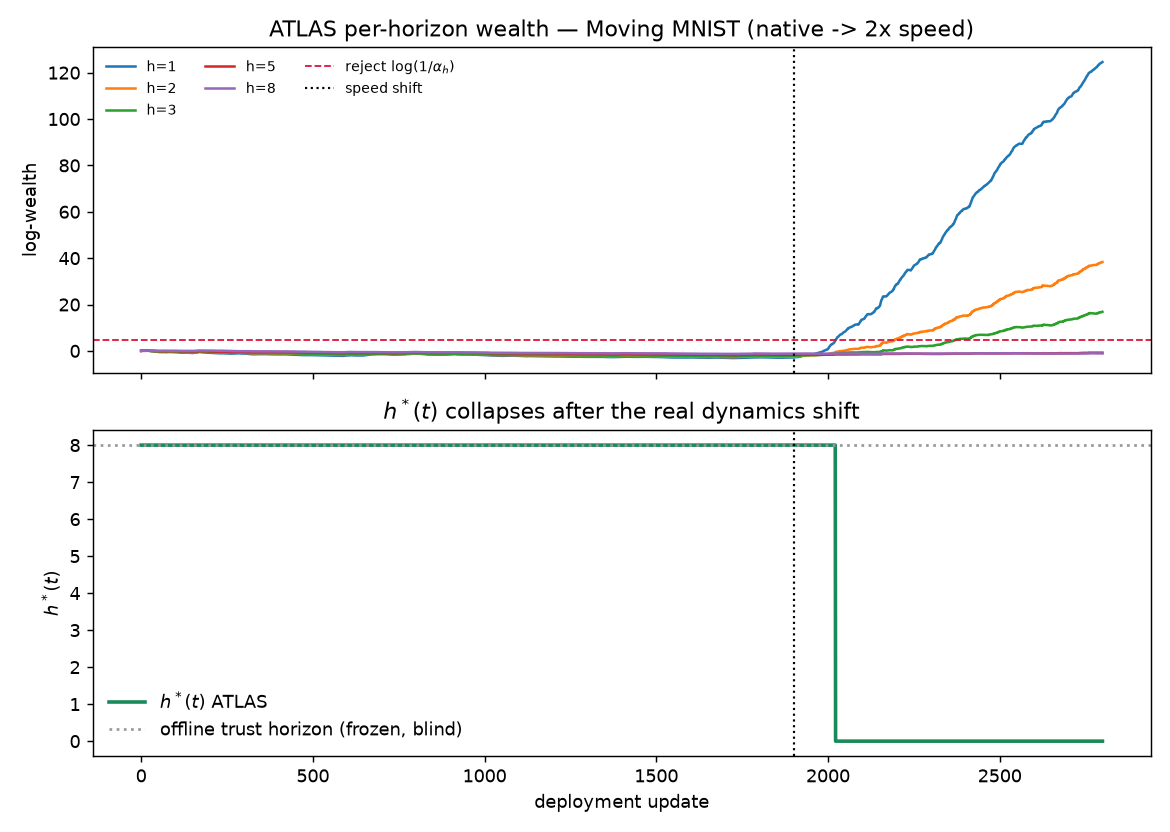
\includegraphics[width=\textwidth]{figures/mnist_frontier.png}\caption{Moving MNIST (speed).}\end{subfigure}\hfill
\begin{subfigure}{0.32\textwidth}
\includegraphics[width=\textwidth]{figures/kth_frontier.png}\caption{KTH walking$\to$running.}\end{subfigure}\hfill
\begin{subfigure}{0.32\textwidth}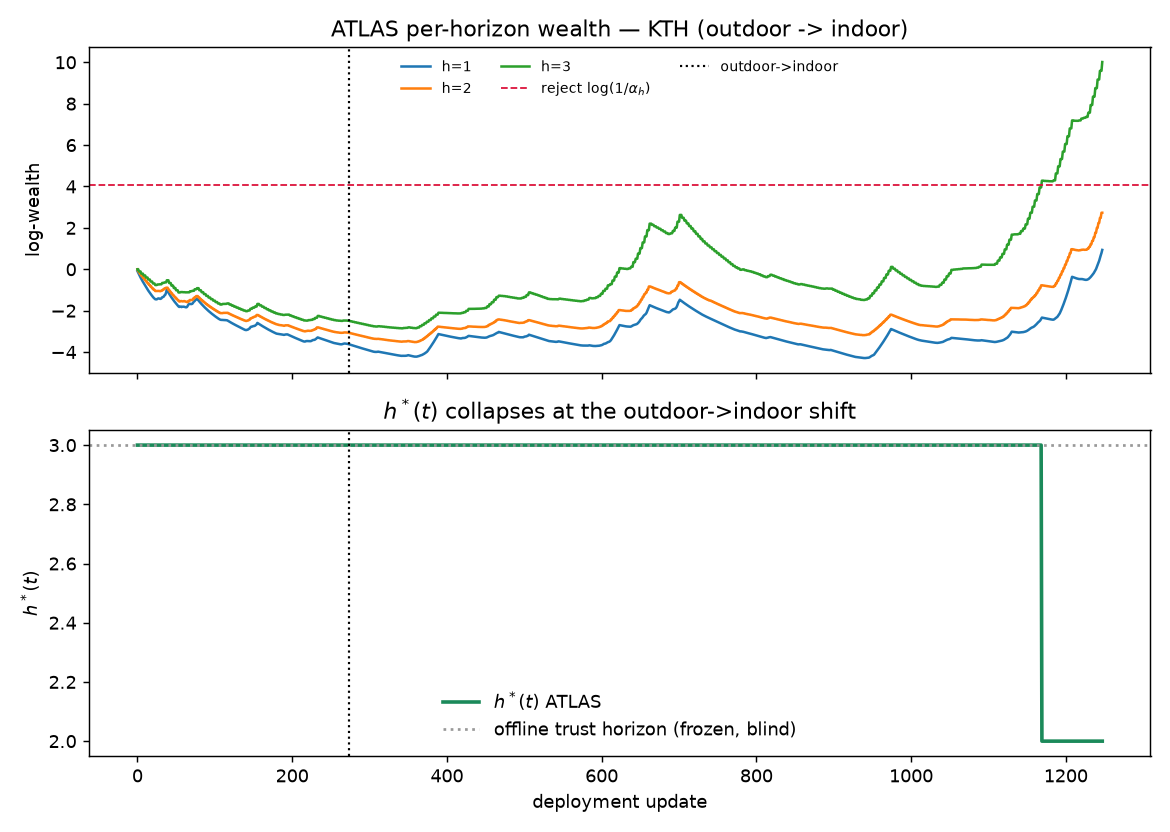
\includegraphics[width=\textwidth]{figures/kth_domain_frontier.png}\caption{KTH outdoor$\to$indoor.}\end{subfigure}
\caption{Real-data frontier collapse under three distinct shifts. In every case the per-horizon
wealth is flat during the in-distribution period (valid), and $\hstar(t)$ collapses when the shift
opens---fully for the two dynamics shifts, partially for the subtle domain shift.}
\label{fig:real}
\end{figure}

\subsection{Learned neural world models on GPU}\label{sec:exp-gpu}

Finally we replace the linear world model with \emph{learned neural} world models behind the
identical \texttt{encode/predict/excess\_stream} interface, run on an NVIDIA T4 GPU, to show that
ATLAS's guarantees are indifferent to model class.

\begin{itemize}\itemsep3pt
\item \textbf{Convolutional-autoencoder world model on Moving MNIST} (a Dreamer-like latent
model). The wealth is flat during the native period; $\hstar$ collapses $3\to0$ after the $2\times$
speed shift (Figure~\ref{fig:gpu}, left). ATLAS's guarantees hold behind a genuinely learned model.
\item \textbf{JEPA-style world model on KTH walking$\to$running.} A frozen ImageNet ResNet-18
encoder (PCA-reduced) with a learned latent-dynamics network generalizes across subjects, so the
in-distribution walking excess is low and stable ($\approx0.1$ at $h=1$) while running is clearly
separated ($\approx1.1$). $\hstar=3$ holds through the entire walking period (a valid null) and
collapses to $0$ once running begins (Figure~\ref{fig:gpu}, right). This experiment also isolates a
practical lesson: a representation that generalizes across the nuisance factors of the deployment
(here, subject identity) is what makes the certificate clean on real video; a stronger world model
such as a full DreamerV3 RSSM drops in behind the same interface.
\end{itemize}

\begin{figure}[t]\centering
\begin{subfigure}{0.49\textwidth}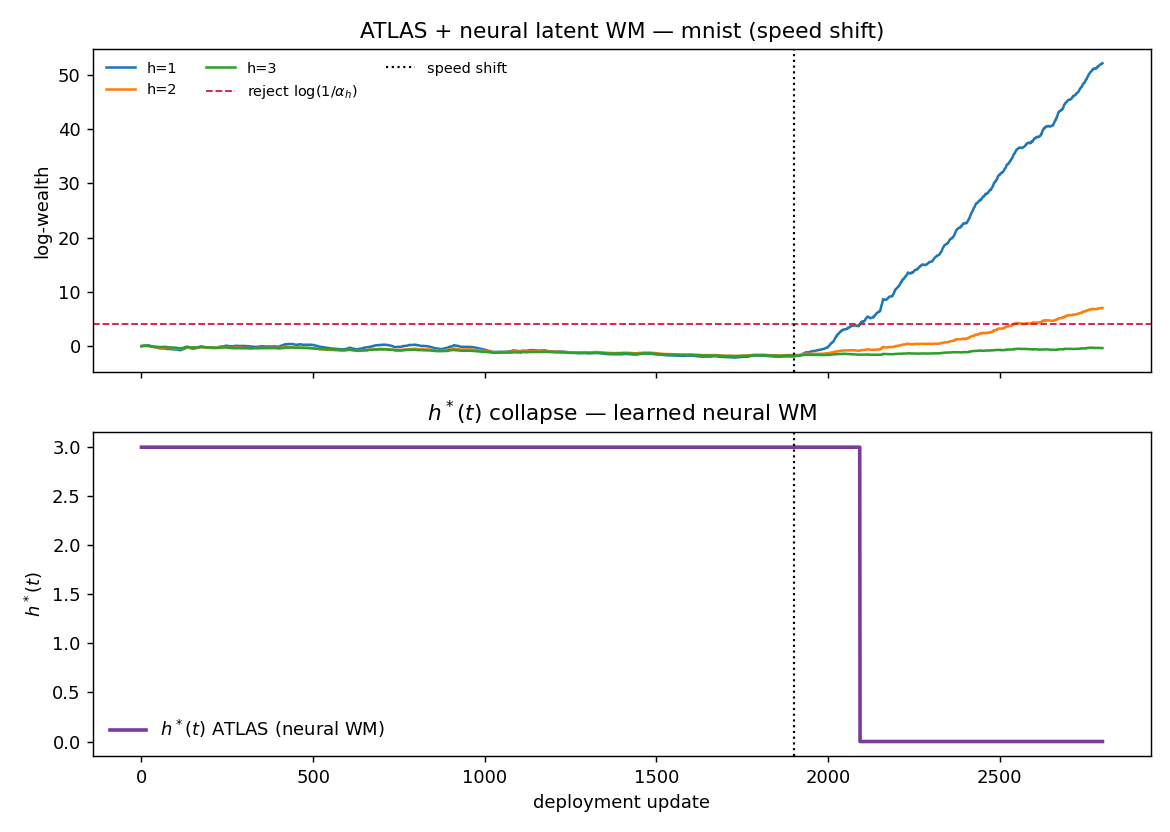
\includegraphics[width=\textwidth]{figures/neural_mnist_gpu.png}\caption{Conv-autoencoder WM, Moving MNIST (speed).}\end{subfigure}\hfill
\begin{subfigure}{0.49\textwidth}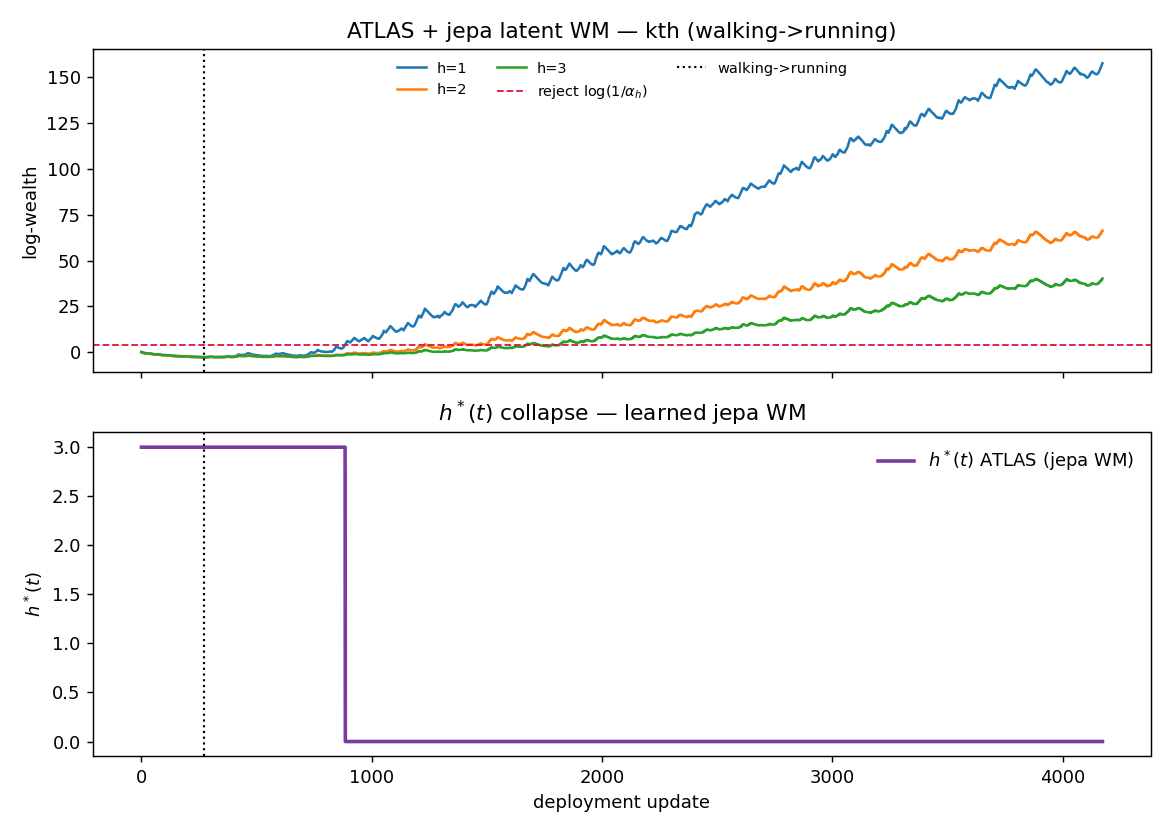
\includegraphics[width=\textwidth]{figures/neural_kth_jepa_gpu.png}\caption{JEPA WM, KTH walking$\to$running.}\end{subfigure}
\caption{ATLAS monitoring \emph{learned neural} world models on a GPU: a valid in-distribution null
(flat wealth) followed by $\hstar(t)$ collapse at the shift, for both a conv-autoencoder and a
JEPA-style model.}
\label{fig:gpu}
\end{figure}

\subsection{Takeaways}
Three findings recur across all tiers. (1) \emph{Validity is never violated:} during every
in-distribution period the wealth is flat and $\hstar$ holds, matching Theorem~\ref{thm:validity}.
(2) \emph{The frontier collapses at the shift,} sharply for dynamics shifts and partially for a
subtle appearance shift, and always before an offline metric would react---indeed the offline
horizon never reacts at all. (3) \emph{The behavior is model-agnostic,} holding for linear,
convolutional-autoencoder, and JEPA-style world models, as the theory requires.

\section{Discussion and limitations}\label{sec:discussion}

ATLAS's validity rests solely on the conditional-mean null under the deployment filtration; it
never invokes independence or exchangeability, which is what makes it sound on the endogenous,
policy-dependent streams that arise in model-based RL. Several honest limitations delineate its
scope and point to future work.

\emph{Exogenous vs.\ fully endogenous evaluation.} Our controlled study uses an exogenous behavior
policy to obtain an \emph{exact} null against which Type-I error can be measured. The
fully policy-in-the-loop regime---where the planner acts through the model under test---is the
ultimate target; the conditional construction is valid there for the same reason, and quantifying
power under closed-loop feedback is natural future work.

\emph{The cost of multi-step validity.} Non-overlapping windows make long horizons genuinely slower
to certify, because they receive fewer effective samples; the interleaved variant
(Appendix~\ref{app:interleave}) mitigates but does not eliminate this. This is an intrinsic
statistical price of honest multi-step testing, not an artifact.

\emph{Certificate quality is bounded by world-model quality.} A low-capacity or overfit world model
produces a non-stationary in-distribution null (its own errors drift across nuisance factors),
which can either mask or spuriously trigger revocation. Our JEPA experiment makes the remedy
concrete: a representation that generalizes across nuisance factors restores a clean certificate.
ATLAS certifies the model it is given; it does not repair a bad one.

\emph{Tolerances are modeling choices.} The $\eps_h$ define what ``faithful'' means. We calibrate
them to the in-distribution level so that ATLAS certifies \emph{departures} from the model's own
baseline; other choices (a fixed absolute tolerance, a risk-derived budget) are equally admissible
and change only the interpretation, not the validity.

\section{Conclusion}\label{sec:conclusion}

We introduced ATLAS, which gives a deployed world model something it has never had: a running,
anytime-valid certificate of faithfulness. The certificate takes the form of a trust horizon
$\hstar(t)$ that collapses precisely when reality drifts from imagination, and it is backed by
three guarantees we proved in full---a uniform no-false-revocation theorem, an anytime-valid
simulation lemma linking certified one-step error to the $h$-step value gap, and an order-optimal
detection-delay bound. The construction is representation- and model-agnostic, requires no
exchangeability, and converts a passive monitor into a planning controller by clipping imagination
depth to the certified horizon. Across a ground-truth simulator, real human-action and video-
benchmark data, and learned neural world models on a GPU, ATLAS behaves exactly as the theory
predicts, while the offline metrics in universal use today stay blind. As world models move from
benchmarks into deployed decision loops, we believe a running, valid faithfulness certificate will
be not a luxury but a requirement, and ATLAS offers a principled foundation for it.

\small
\bibliographystyle{plainnat}
\bibliography{references}

\normalsize
\appendix

\section{Interleaved non-overlapping chains}\label{app:interleave}
For horizon $h$, partition issue times into $h$ offset classes $c\in\{0,\dots,h-1\}$, each a
non-overlapping chain $\{c,c+h,c+2h,\dots\}$ on which residuals are conditionally independent. Run
one e-process $W^{(h,c)}$ per class. Each is valid on its own coarse filtration by
Proposition~\ref{prop:evar}. Testing horizon $h$ by rejecting when \emph{any} class crosses
$H h/\alpha$ (a union bound over the $h$ classes and $H$ horizons) uses every issue time while
retaining validity at level $\alpha$; the cost is an additional $\log h$ in the threshold. This
recovers the data efficiency lost to non-overlap at a logarithmic price.

\section{Reproduction details}\label{app:repro}
The reference implementation (\texttt{atlas/}: proper scores; the mixture-betting e-process, the
two-sided betting confidence sequence, and the Shiryaev--Roberts e-detector; the horizon-indexed
frontier) and the controllable latent simulator are provided, along with all experiment scripts.
Synthetic study: \texttt{python -m experiments.run\_all} regenerates
Table~\ref{tab:validity} and Figures~\ref{fig:teaser},~\ref{fig:validity}. Real data:
\texttt{python -m experiments.real\_data.download} then the \texttt{exp\_mnist},
\texttt{exp\_kth}, and \texttt{exp\_kth\_domain} scripts produce Figures~\ref{fig:frames},
\ref{fig:real}. GPU neural world models: \texttt{python -m experiments.gpu.run\_neural
--dataset kth --model jepa} (auto-selects CUDA) produces Figure~\ref{fig:gpu}; the GPU runs in
this paper were executed on a Colab T4. The verified bibliography is in \texttt{references.bib};
extended derivations accompany the code in \texttt{docs/}.

\end{document}
